\documentclass{llncs}

\usepackage{url}
\usepackage[pdftex]{graphicx}
\usepackage{listings}
\usepackage{verbatim}
\usepackage[lined,linesnumbered,algochapter]{algorithm2e}
\usepackage{tikz}
\usetikzlibrary{arrows,automata}
\usepackage{xspace}
\usepackage {pdfsync}

\usepackage{ngerman}
\usepackage[ngerman, english]{babel}
\usepackage{bibgerm,cite}       % Deutsche Bezeichnungen, Automatisches Zusammenfassen von Literaturstellen
\usepackage[ngerman]{varioref}  % Querverweise

\setcounter{secnumdepth}{2}
\setcounter{tocdepth}{3}

% define custom macros for specific formats or names
\newcommand{\uml}[1]{\texttt{#1}}
\newcommand{\cd}{\textsf{Class Diagram}}

\begin{document}
\pagestyle{plain}
\pagenumbering{roman}

\title{Towards Systematic Mutations for and with ATL Model Transformations\footnote{This work has been created in the context of the course ``188.952 Advanced Model Engineering (VU 2,0)'' in SS15.}}


%&&&&&&&&&&&&&&&&&&&&&&&&&&&&&&&&&&&&&&&&&&&&&&&&&&&&&&&&&&&&&&&&&&&&&&&&
% Name and address of the author
%&&&&&&&&&&&&&&&&&&&&&&&&&&&&&&&&&&&&&&&&&&&&&&&&&&&&&&&&&&&&&&&&&&&&&&&&
\author{Patrick Sommer\inst{1} and Carola Gabriel\inst{2} and Martin Keiblinger\inst{3}}

\institute{Mautner Markhof-Gasse 58/4/31, 1110 Wien \\ \email{e0925011@student.tuwien.ac.at} \\ MatrNr.: 0925011
\and
Mustergasse 54/4/3, 1030 Wien \\ \email{matthias@tuwien.ac.at} \\ MatrNr.: 0426553
\and
Mustergasse 54/4/3, 1030 Wien \\ \email{matthias@tuwien.ac.at} \\ MatrNr.: 0426553
}

\maketitle

\begin{abstract}

This abstract summarizes the content of this paper in about 70 to 150 words. \dots
\end{abstract}

%&&&&&&&&&&&&&&&&&&&&&&&&&&&&&&&&&&&&&&&&&&&&&&&&&&&&&&&&&&&&&&&&&&&&&&&&
% Table of contents
% Activate or deactivate this according to the guideline instructor
%&&&&&&&&&&&&&&&&&&&&&&&&&&&&&&&&&&&&&&&&&&&&&&&&&&&&&&&&&&&&&&&&&&&&&&&&
\tableofcontents
%\thispagestyle{plain}
\newpage

\pagenumbering{arabic}

\section{Introduction}

The broader goal of this work is to create an introduction to a specific field of software testing. Software testing is a process, or a series processes engineered to check if a program does what it is designed to do and that id does not do anything unintended.\cite{Myers:2004} Model based testing (MBT) is a variant of testing. Test cases are not written by the programmer directly. The programmer creates a model of the requirements and in a second step the test cases are generated on base of the model.\cite{Utting:2012}

Mutation testing is a fault-based testing technique. It applys changes to the input and creates a mutant. A mutant represents a faulty program. In the best case these changes, which are applied by the mutator, represent mistakes a programmer would make.\cite{mutationssurvey:yue}

The basic idea is of mutation testing is not to test the resulting software itself but the test cases. Good test cases should be able to identify mutants. Identifying means recognizing differing results of the original system under test (SUT) or mutants.\cite{MatMottu2006}

The process of mutation testing consists of these components:
\begin{itemize}
	\item \textit{Test data} as input for the original programm P and its mutants.
	\item The original program \textit{P}
	\item The \textit{mutants} of P.
	\item An \textit{oracle} which is able to decides if results differ and which is therefore able to identify mutants.
\end{itemize}

\begin{figure}
	\centering
	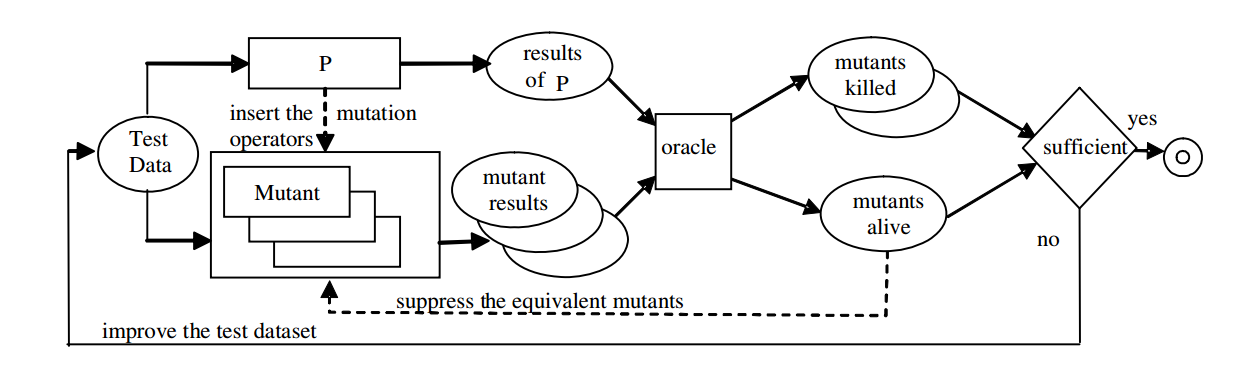
\includegraphics[width=0.7\textwidth]{figures/Mutation_Process}
	\caption{The mutation testing workflow contains a feedback loop.\cite{MatMottu2006}}
	\label{fig:Mutation_Process}
\end{figure}

The mutation score is the ratio of the number of detected faults over the total number of the sseeded faults. It is a way to meassure how effective an input test set is.\cite{mutationssurvey:yue}

This report discusses a technique to create an mutator which doesn't work on model base but on meta-models. The purpose is to automate the creation of mutations by creating generic mutators.

\section{General}

Model transformations play an important role in the Model Driven Engineering
(MDE) approach. Developing model transformation definitions is expected to
become a common task in model driven software development. \cite{atl:frederic}
In this part of the paper we want to explain the basics of the requirements we needed for Mutations for and with ATL Model Transformations.

\subsection{Model transformation}
Model transformation is an important technique in software development, espacially in Model-Driven Software Development (MDSD) and Model-Driven Software Development (MDA). There exists different types of model transformations like Model-To-Model Transformation and Model-To-Text Transformation.  

\subsection{ATL}
ATL is a model transformation language containing a mixture of declarative and
imperative constructs. ATL is applied in the context of the
transformation pattern shown in \label{fig:overview_atl}. In this pattern a source model Ma is transformed into a target model Mb according to a transformation definition mma2mmb.atl written in the ATL language. The transformation definition is a model conforming to the ATL metamodel. All metamodels conform to the MOF.
ATL is a hybrid transformation language. It contains a mixture of declarative
and imperative constructs. We encourage a declarative style of specifying transformations. The declarative style of transformation specification has a number of advantages. It is usually based on specifying relations between source and target patterns and thus tends to be closer to the way the developers intuitively perceive a transformation. This style stresses on encoding these relations and hides the details related to selection of source elements, rule triggering and ordering, dealing with traceability, etc. Therefore, it can hide complex transformation algorithms behind a simple syntax.\cite{atl:frederic}

\begin{figure}
	\centering
	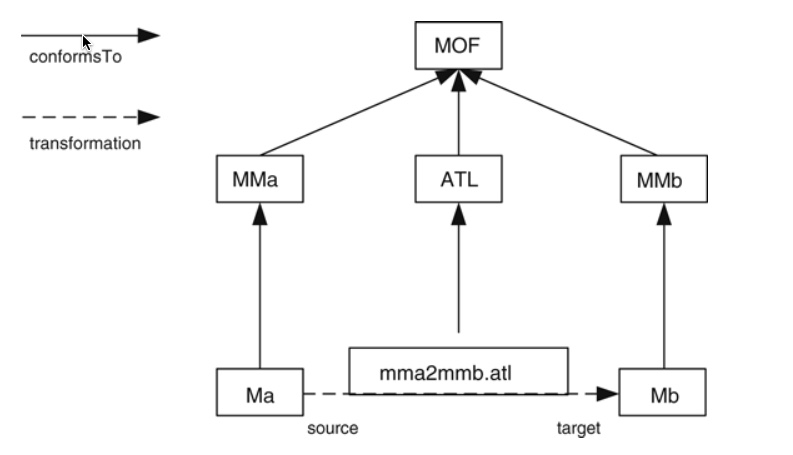
\includegraphics[width=0.7\textwidth,natwidth=610,natheight=642]{figures/Overview_ATL.jpg}
	\caption{Overview of the ATL transformational approach}
	\label{fig:overview_atl}
\end{figure}~\cite{atl:frederic}

\begin{figure}
	\centering
	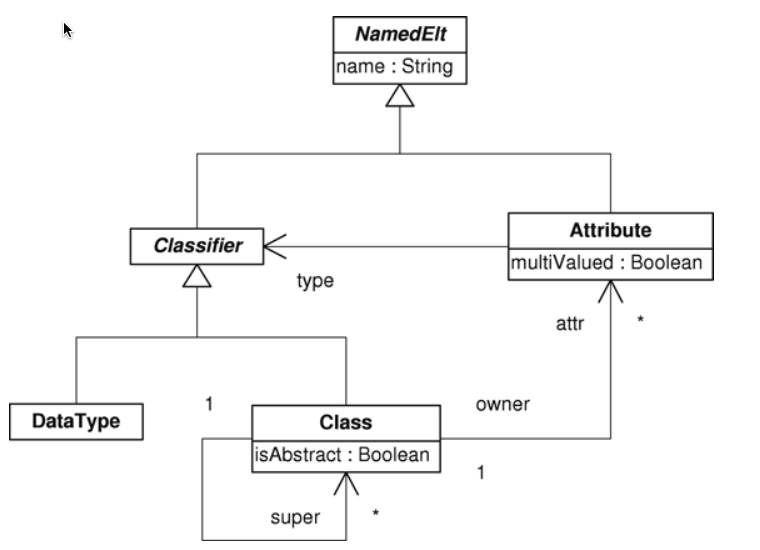
\includegraphics[width=0.7\textwidth,natwidth=610,natheight=642]{figures/Class_metamodel.jpg}
	\caption{Class metamodel}
	\label{fig:class_metamodel_atl}
\end{figure}~\cite{atl:frederic}

\begin{figure}
	\centering
	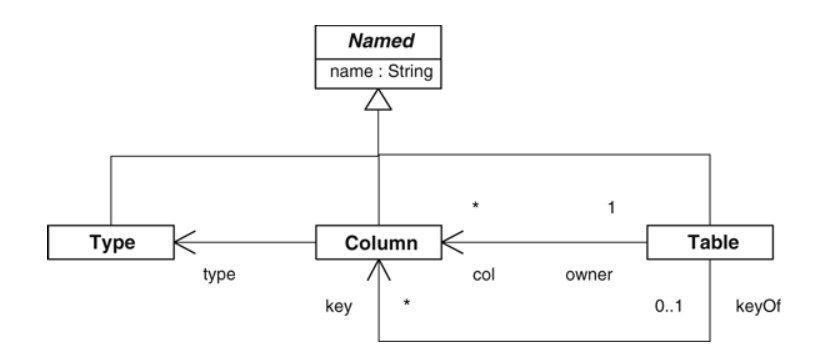
\includegraphics[width=0.7\textwidth,natwidth=610,natheight=642]{figures/Relational_metamodel.jpg}
	\caption{Relational metamodel}
	\label{fig:relational_metamodel_atl}
\end{figure}~\cite{atl:frederic}

In the following you can see a short example of a ATL transformation:
\begin{verbatim}
//Start Program
module Entities2Forms;
create OUT : Forms from IN : Forms;

rule EntityModel2FormModel {
	from
		em : Forms!EntityModel
	to 
		fm : Forms!FormModel (
		)
}
//End Program
\end{verbatim}

This ATL file shows a tranformation Entities2Form. The source model is the 'IN'
model and the target model is 'OUT'. The rule mapped the elements EntityModel to
FormModel. 


\subsection{High Order Transformations}
High Order Transformations are defined in some special languages of model
transformations. That means that the model transformation is itself a model. The
input and output models are also themselves transformation models. 

\begin{figure}[tb]
	\centering
	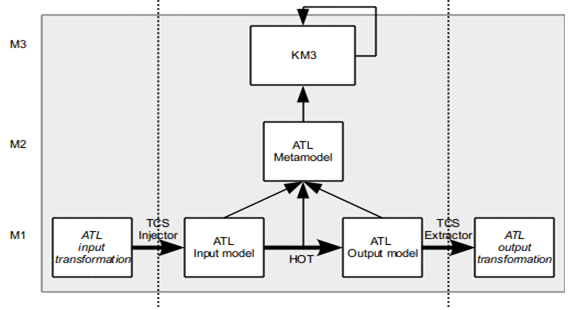
\includegraphics[width=0.7\textwidth,natwidth=610,natheight=642]{figures/HOT.png}
	\caption{Sample schema of a HOT for transformation modification in ATL}
	\label{fig:samplefigure_pdf}
\end{figure}~\cite{misc:ModelingLanguages}

\section{Implementation}

For working with LaTeX you can take advantage of a variety of books and free introductions and tutorials on the internet. A competent contact point for LaTeX beginners is the LaTeX Wikibook, which is available under \url{http://en.wikibooks.org/wiki/LaTeX}. 

The following sections give examples of the most important LaTeX environments and commands.

\subsection{Tables}

Tables have to be realized with the help of the \textit{table} environment. Tables shall be sequentially numbered for each chapter and described in terms of a short caption (cf. Table~\ref{tab:diplomaseminar}).

\begin{table}[htb]
	\centering
	\begin{tabular}{|l|c|c|}
		\hline \textbf{Name} & \textbf{Date} & \textbf{Title} \\
		\hline
		\hline Mustermann Adam  & 18.5   & T1    \\
		\hline Musterfrau Eva  & 22.6   & T2    \\
		\hline
	\end{tabular}
	\caption{Seminar for Master Students}
	\label{tab:diplomaseminar}
\end{table}


\subsection{Figures}

Like tables, figures shall be sequentially numbered for each chapter and described in terms of a short caption). You could either produce your drawings directly inside Latex using PSTricks\footnote{\url{http://tug.org/PSTricks}}, Tikz\footnote{\url{http://sourceforge.net/projects/pgf}}, or any set of macros dedicated to your requirements (cf. Figure~\ref{fig:samplefigure_tikz}). Alternatively, you may include figures prepared in external tools (cf. Figure~\ref{fig:samplefigure_pdf}). Note, to ensure high quality printing, all figures must have at least 300 dpi.

\begin{figure}
	\centering
	\begin{tikzpicture}[->, auto, node distance=2.8cm, semithick]
	  \node[initial, state] (1)		 {$S_1$};
	  \node[state] 		(2) [right of=1] {$S_2$};
	
	  \path (1) edge [bend left]  node {0} (2)
		(1) edge [loop above] node {1} (1)
		(2) edge [bend left]  node {0} (1)
		(2) edge [loop above] node {1} (2);
	\end{tikzpicture}
	\caption{Sample figure}
	\label{fig:samplefigure_tikz}
\end{figure}

\begin{figure}[tb]
	\centering
	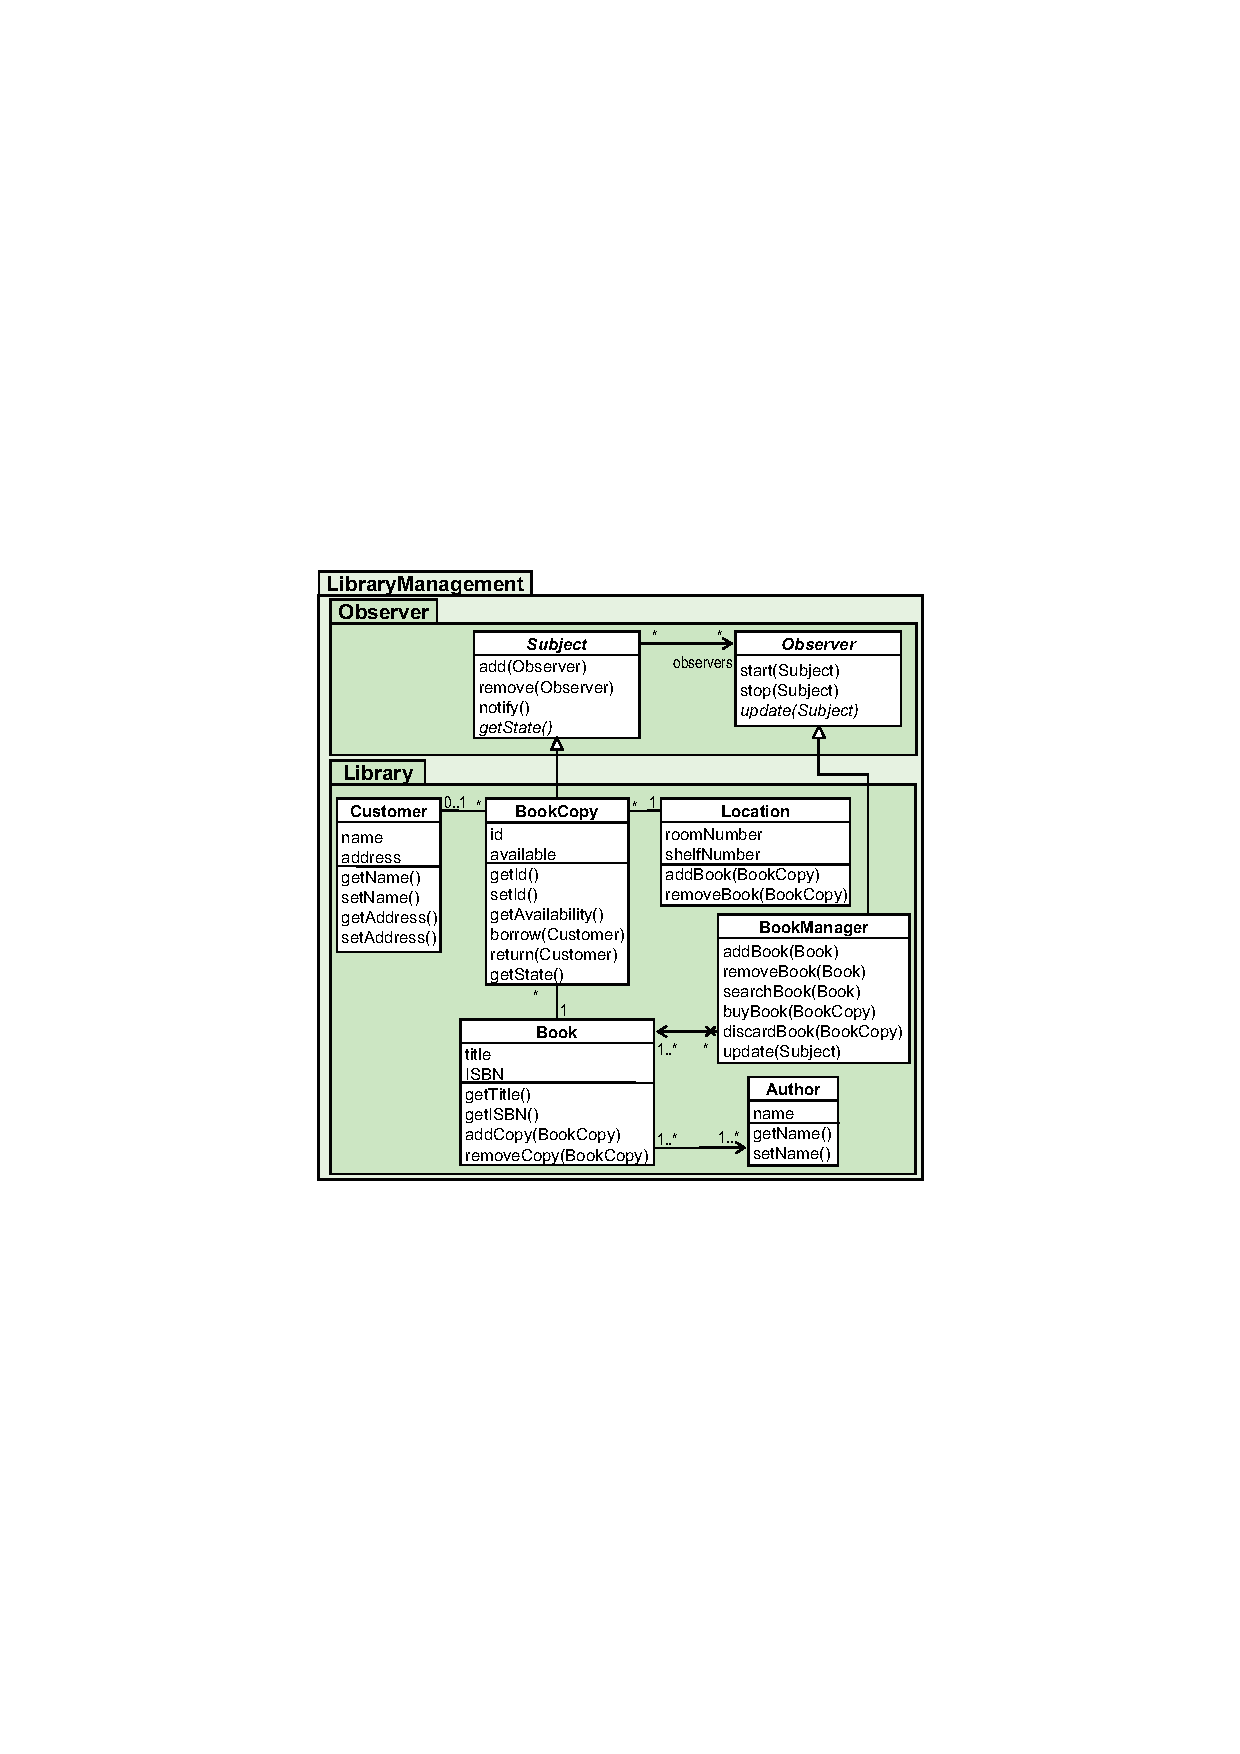
\includegraphics[width=0.8\textwidth,natwidth=610,natheight=642]{figures/figure1.pdf}
	\caption{Sample figure}
	\label{fig:samplefigure_pdf}
\end{figure}


\subsection{Fonts}

When introducing important terms for the first time use \emph{emphasize}. For a consistent look and feel of proper names like {\cd} and {\uml{Observer}} pattern you may define macros in the main document \texttt{thesis.tex}.

\subsection{Code}

For short code fragments use the \textit{verbatim} environment.

\begin{verbatim}
//Start Program
System.out.println("Hello World!");
//End Program
\end{verbatim}

A much better alternative is the \textit{algorithm} environment (cf. Algorithm~\ref{alg:samplealgorithm}). This environment offers special formatting features for loops, operations and comments.

\begin{algorithm}[t]
\SetKwData{Left}{left}
\SetKwData{This}{this}
\SetKwData{Up}{up}
\SetKwFunction{Union}{Union}
\SetKwFunction{FindCompress}{FindCompress}
\SetKwInOut{Input}{input}
\SetKwInOut{Output}{output}

\Input{A bitmap $Im$ of size $w\times l$}
\Output{A partition of the bitmap}

\BlankLine

\emph{special treatment of the first line}\;
\For{$i\leftarrow 2$ \KwTo $l$}{
\emph{special treatment of the first element of line $i$}\;
\For{$j\leftarrow 2$ \KwTo $w$}{\label{forins}
\Left$\leftarrow$ \FindCompress{$Im[i,j-1]$}\;
\Up$\leftarrow$ \FindCompress{$Im[i-1,]$}\;
\This$\leftarrow$ \FindCompress{$Im[i,j]$}\;
\If(\tcp*[r]{O(\Left,\This)==1}){\Left compatible with \This}{\label{lt}
\lIf{\Left $<$ \This}{\Union{\Left,\This}}\;
\lElse{\Union{\This,\Left}\;}
}
\If(\tcp*[r]{O(\Up,\This)==1}){\Up compatible with \This}{\label{ut}
\lIf{\Up $<$ \This}{\Union{\Up,\This}}\;
\tcp{\This is put under \Up to keep tree as flat as possible}\label{cmt}
\lElse{\Union{\This,\Up}}\tcp*[r]{\This linked to \Up}\label{lelse}
}
}
\lForEach{element $e$ of the line $i$}{\FindCompress{p}}
}
\caption{Sample algorithm}\label{alg:samplealgorithm}
\end{algorithm}

\section{Bibliographic Issues}

\subsection{Literature Search}

Information on online libraries and literature search, e.g., interesting magazines, journals, conferences, and organizations may be found at \url{http://www.big.tuwien.ac.at/teaching/info.html}.

\subsection{BibTeX}

BibTeX should be used for referencing.

The LaTeX source document of this pdf document provides you with different samples for references to journals~\cite{jour:B2BServices}, conference papers~\cite{proc:TheWebMLApproach}, books~\cite{book:umlatwork}, book chapters~\cite{incoll:ErhardKonrad1992}, electronic standards~\cite{man:BPEL}, dissertations~\cite{phdthesis:manuelWimmer}, masters' theses~\cite{mast:AUMLProfile}, and web sites~\cite{misc:BIGWebsite}. The respective BibTeX entries may be found in the file \texttt{references.bib}. For administration of the BibTeX references we recommend \url{http://www.citeulike.org} or JabRef for offline administration, respectively.

\bibliographystyle{acm}
\bibliography{references}

\end{document}
